\section{Modelització del problema}
La pràctica ha estat desenvolupada en \emph{Python} el qual te una estructura de dades molt optimitzada
i integrada al llenguatge que és el diccionari\footnote{\url{http://docs.python.org/library/stdtypes.html\#dict}}
el qual dona suport a la majoria d'estructura de dades de la pràctica.

\subsection{Representació de les dades}
Per la representació de les dades es fan servir 3 classes: passatger, conductor i estat.

On estat es l'estat requerit per les llibreries del AIMA. Passatger i conductor han estat
definits per facilitar l'elaboració de la pràctica.

\subsubsection{Passatger}
Cada passatger ve representat amb un identificador i els punts d'origen i destí tots ells són
camps invariables durant l'execució.

Assosciat a aquesta classe simplement hi ha els mètodes per obtenir el valors de dits camps.

\subsubsection{Conductor}
El conductor és una classe que hereda del passatger, així doncs també té el camp que l'identifica
el seu origen i destí. A més també té una capacitat màxima.
Per altra banda el conductor també inclou una llista dels noms dels passatgers que transportarà
durant tota la seva ruta.

Per gestionar aquesta classe són necessaris diveros mètodes més complicats que simples \emph{settes} i \emph{gettes}.
En primer lloc hi ha una funció \texttt{pickupPassenger} per recollir un passatger, aquesta afegeix el passatger
a la llista de passatgers a transportar. De manera complementària te \texttt{leavePassenger} per deixar un 
passatger.

Per tal de sabre quina és la ruta que fa el conductor hi ha la funció \texttt{getRoute} la qual
fa una ordenació dels punts clau (\texttt{checkpoints}) per on es passa i registra a cada punt si es
l'origen del condcutor, l'origen d'un passatger, el destí del passatger o el destí del condcutor. Així
doncs un ruta tindria l'aspecte seguent: 

\begin{minted}[frame=lines, fontsize=\codeSize]{python}

     [[[33, 44], "DriverOrigin", "D-0000"],
      [[34, 45], "PickupPassenger", "P-00001"],
      [[55, 65], "LeavePassenger", "P-00001"],
      [[57, 70], "DriverDestination", "D-0000"]]
\end{minted}

Associat a una ruta ens interessa sabre la distància que recorre, per això hi ha la funció \emph{getKm}
que torna tal valor.

En aquest punt s'ha de tenir amb compte com es generen les rutes ja que això infuleix directament en
si un passatger pot ser tranportat o no.

La manera òptima en quan a recorregut seria fent un viatjant
de comerç entre tots els punts per on s'ha de passar tinguent amb compte dos factors:
Un cop s'agfa un passatger s'ha de introudir a la llista de punts el seu destí.
S'ha de vigilar de no agafar més passatgers del que pot transportar el vehicle
abans de deixar-ne algun.

Aquest problema tot hi ser TSP pot dur-se a terme ja que un conductor no sol transportar més de 3
persones en una ruta la qual cosa suposen un total de 8 punts. Així i tot el càlcul de la ruta
es la funció més emprada durant l'execució i interessa minimitzar el seu cost.

Per tal de simplificar-ho en lloc del viatjant de comerç es van cercant els punts més propers de
manera imediata. Es pot observar que si el cotxe és ple primer es deixa algun dels passatgers
abans d'anar a cercar-ne un de nou.

\begin{minted}[frame=lines, fontsize=\codeSize]{python}
  def getRouteHeuristic(self, state):
    ## Dictionary of tuplas name-originPoint pointing destinations
    # i.e. { ("P-0001", [34, 45]) : [22, 56] }
    checkpoints = {}

    ## Dictionary of carried passengers pointing to their destinations
    # i.e { ("P-0001" : [22, 56] }
    checkpointsDest = {}

    ## List of tuples [point, event, name]
    # i.e. [[34, 45], "PickupPassenger", "P-0001"]
    route = []

    # Inserting all origin points
    for p in self.__passengers:
      src = state.getPassengers()[p][0].getOrigin()
      dst = state.getPassengers()[p][0].getDestination()
      checkpoints[(p, src)] = dst

    current = (self.getOrigin(), "DriverOrigin", self.getName())
    route.append(current)
    npass = 0
    routeDist = 0
    while checkpoints or checkpointsDest:
      # Searching nearst point
      dmin = INTMAX
      nearest = None

      for (n, p) in checkpointsDest.iteritems():
        d = distance(current[0], p)
        if d < dmin:
          dmin = d
          nearest = p
          name = n

      if npass < self.__maxSpace:
        for (n, p) in checkpoints.keys():
          d = distance(current[0], p)
          if d < dmin:
            dmin = d
            nearest = p
            name = n

      if (name, nearest) in checkpoints:
        checkpointsDest[name] = checkpoints[(name, nearest)]
        checkpoints.pop((name, nearest))
        event = "PickupPassenger"
        npass += 1
      else:
        event = "LeavePassenger"
        checkpointsDest.pop(name)
        npass -= 1
        
      routeDist += d
      current = (nearest, event, name)
      route.append(current)
    
    route.append((self.getDestination(), "DriverDestination", self.getName()))
    self.calculatedRouteWeight = routeDist + distance(route[-2][0], route[-1][0])
    return route
\end{minted}

Donat també que hi ha poc punts i son molt dispersos aquesta aproximació, en el nostre cas,
dona un resultat acceptable estalviant temps d'execució.

El cost d'aquesta si $P$ fos el número de passatgers seria $((P+1) \times 2)^2$, el més u
es per afegir els conductors i es multiplica per dos perque cada un té dos punts.

No obstant en l'argorisme es van llevant els punts per on ja s'ha passat, per tant
en cada iteració el numero de punts pendents decreix. Per altra banda incialment nomes tenim
visibilitat dels origens i anam afegint els destins a mesura que s'arriba els origens (a que alhora son trets).
A tot això s'ha d'afegir que mai es tenen mes de 3 destins ja que sino significaria
que el cotxe has escedit la seva capacitat.

Així doncs el temps d'execució d'obtenir la ruta roman més que acceptable.

\subsubsection{Ciutat}
La citutat en si no requereix representació, no té perquè estar guardara en memòria ja que senzillament
es pot guardar a cada passatger i conductor el seu punt d'inici i de destí com dues tuples \emph{XY}.

Per tant la so\lgem ució no és més que el conjunt de rutes dels conductors que formen part de l'estat.

\subsubsection{Estat}
L'estat ve determinat per un diccionari de conductors i un de passatgers (fig. \ref{diccionarisPssDrv}).
Ambdós diccionars estan indexats per els noms de passatger i conductor respectivament però contenen coses diferents.

El diccionari de conductors conté un punter a cada objecte conductor mentre el diccionari
de passatgers conté una tupla amb l'objecte del passatger i el nom del conductor que el transporta.

El fet de tenir un diccionari de passatgers es informació redundant però així es pot sabre
amb qui va un passatger en temps mig de $O(1)$ en lloc de $O((n_{passatgers} + n_{conductors})/2)$ 
si haguéssim de recorrer tots els conductors i comprovar tots els passatgers que transporten.

\begin{figure}[H]
\begin{center}
 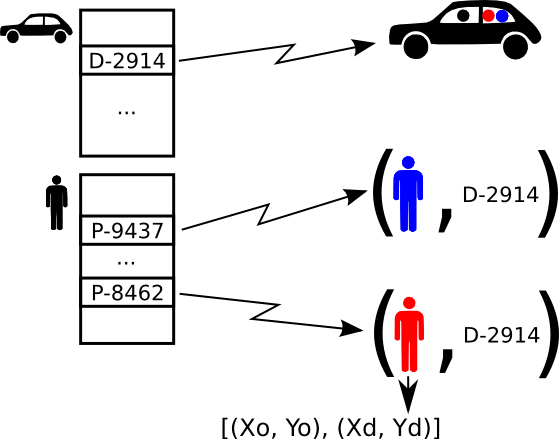
\includegraphics[width=0.6\textwidth]{figures/diccionarisPssDrv.png}
 \caption{Estructures de dades dins l'estat}
 \label{diccionarisPssDrv}
\end{center}
\end{figure}


\subsection{Estat inicial}
Per la generació de l'estat inicial s'han contemplat dues maneres de fer-ho. En cap de les dues es contempla
la possiblitat de que algun passatger no sigui transportat per algun conductor. \textbf{Com a invariant durant
tota l'execució tot passatger es transportat per algun conductor.}

També en ambdós casos l'assignació d'un passatger a un conductor és aleatoria.

A continuació trobm les dues maneres d'inicialitzar el problema.

\subsubsection{Per saturació de conductors - \emph{fullFirst}}
En aquesta inicialització del problema es recorren tots els passatgers assignant-los a conductors. No es passa
al següent conductor fins que aquest no arriba a un determinat nombre prefixat. Així doncs a un conductor no se
li assignara un passatger fins que tots els anteriors no siguin \emph{saturats}. Més endavant veurem
que el control de si el cotxe esta massa ple en algun instant es detectat per l'heurístic, així doncs
durant l'execució de la pràctica hi poden haver conductors que transportin més passatgers dels que
caben al vehicle.

% \begin{figure}[H]
% \begin{center}\label{fullFirst}
%  \includegraphics[width=0.6\textwidth]{figures/fullFirst.png}
%  \caption{Inicialització full first}
% \end{center}
% \end{figure}


Amb aquesta inicialització cap passatger queda sense transport, molt possiblement els condcutros escedeixin
la seva distància màxima i gairebé sempre hi haurà conductors que no transportin ningu.
Dit esces de la capacitat màxima es veura reflectit molt negativament a l'heurístic.


\subsubsection{Evitant deixar conductors buits - \emph{allOneFirst}}
L'altre alternativa plantejada per la inicialització és recórrer tots els passatgers i assignar-los a conductors
de tal manera que no s'assigni un segon passatger a un conductor mentre hi hagin conductors buits.
D'aqueta manera s'afavoreix que les rutes dels conductors siguin més curtes i que hagi més
gent conduint.

TODO diagrama

\subsection{Operadors de transformació}
S'han establert quatre operadors de transformació agrupats en dos conjunts. Així doncs en la fase d'experimentació
es triara si l'agafa el conjunt 1 o el conjunt 2.

En el codi és pot veure que els operadors són funcions que retornen un iterador \texttt{yield} en \emph{pyhton},
de tal manera que així s'evita tenir-los tots en memòria i a cada crida de la funció es retorna el següent.

\subsubsection{Conjunt 1}
El conjunt 1 preten ser un conjunt minimalista de les operacions més bàsiques que podem fer amb el nostre plantejament
de la pràctica.
\subsubsection{Canvi de passatger de vehicle}
Aquest operador senzillament canvia un passatger de un vehicle a un altre, això vol dir que si en un estat
tenim $P$ passatgers i $C$ conductors podem generar un total de $P\times(C-1)$ estats successors.

\begin{minted}[frame=lines, fontsize=\codeSize]{python}
def genPassengerSwitches(self, state):
  #Gens all the passenger changes (gens at most nPassengers*nDrivers states)
  for p in state.getPassengers():
    currentDrv = state.whoPickuped(p)  
    for d in state.getDrivers().iteritems():
      if d[0] != currentDrv :
	#Switch passenger to this driver
	newState = copy(state)
	newState.setDrivers(copy(state.getDrivers()))
	newState.setPassengers(copy(state.getPassengers()))
	newState.switchPassenger(p, d[0])
	yield ("sw", newState)
\end{minted}

Cal notar que aquest operador com a efecte pot anar buidant un conductor fins que es quedi sense passatgers,
cos útil quan també disposam del següent operador.

\subsubsection{Eliminació d'un conductor buit}
Aquest operador consisteix en e\lgem imiar un conductor que no transporta ningú i posar-lo com a passatger
en un dels altres conductors. Així doncs si en un estat tenim $C$ conductors $B$ dels quals són buits
podem generar $B*(C-1)$ estats.

\begin{minted}[frame=lines, fontsize=\codeSize]{python}
def genSoftDriverDegradations(self, state):
  #Gens all the empty driver deletions
  for d in state.getDrivers().itervalues():
    if d.isEmpty():
      for carrier in state.getDrivers().iteritems():
	if carrier[0] != d.getName():
	  newState = copy(state)
	  newState.setDrivers(copy(state.getDrivers()))
	  newState.setPassengers(copy(state.getPassengers()))
	  newState.degradateDriver(d.getName(), carrier[0])
	  yield ("dgrd", newState)
	  break
\end{minted}

En la so\lgem ució els passatgers que eren originalment conductors tenen el nom de la manera \texttt{PDnnnn},
on s'ha substiutit el guió \texttt{P-nnnn} per una \emph{D} de \emph{driver}.

\subsubsection{Conjunt 2}
A diferència del primer conjunt d'operadors aquest està format per operacions compostes.

\subsubsection{Intercanvi d'un passatger per un altre}
En aquest operador s'intercanvia un passatger per un altre que no sigui del mateix conductor.
Així doncs si tenim $P$ passatgers i $F$ conductors no buits podem generar $P \times (F-1)$ estats. 

\begin{minted}[frame=lines, fontsize=\codeSize]{python}
  def genPassengerSwaps(self, state):
    it = 0
    ltemp = list(state.getPassengers())
    for p1 in ltemp:
      for p2 in xrange(it,len(ltemp)):
        newState = copy(state)
        newState.setDrivers(copy(state.getDrivers()))
        newState.setPassengers(copy(state.getPassengers()))
        newState.swapPassengers(p1,ltemp[p2])
        yield ("swap", newState)
      it += 1
\end{minted}

Hem de notar aque amb aquest operador no es buiden vehicles però tampoc se n'omplen de nous.
Així doncs aquesta funció amb una inicialització \emph{full first} podria semblar que no ha de funcionar
gaire bé ja que hi hauria tot un conjunt de conductors buits que sols es transportarien a ells mateixos.


\subsubsection{Eliminació d'un conductor no buit}
Aquest operador s'elimina un conductor qualsevol i es distribueixen els seus passatgers i ell mateix
en diferents conductors de manera aleatoria.

\begin{minted}[frame=lines, fontsize=\codeSize]{python}
  def genHardDriverDegradations(self, state):
    #Gens all the driver deletions inserting it in the first not full driver.
    for d in state.getDrivers().itervalues():
      for carrier in state.getDrivers():
        if carrier != d.getName():
          newState = copy(state)
          newState.setDrivers(copy(state.getDrivers()))
          newState.setPassengers(copy(state.getPassengers()))
          # Distribution of passengers in other drivers
          for p in d.getPassengers():
            for anotherDriver in newState.getDrivers():
              if anotherDriver != d.getName():
                newState.switchPassenger(p, anotherDriver)
          # Puts the old driver as a passenger with the carrier driver.
          newState.degradateDriver(d.getName(), carrier)
          yield ("dgrd", newState)
          break
\end{minted}

En principi pot semblar irracional llevar un conductor que podria estar ple però ha de ser l'heurístic
que valori si realment aquell canvi ha valgut la pena.
A l'apartat anterior es mencionava que aquest conjunt d'operadors podia no presentar bons resultats
combinat amb una inicialització \emph{full first} ja que els conductors buits nomes es transportarien
a ells mateixos. El cas es que amb aquest segon operador es dissolen aquests conductors saturats
repartit a tothom per les demes ja siguin buits o plens. Tal vegada inicialment els resultats siguin
mes dolents pero aquestes dissolucions donen mes moviment als passatgers que podrien acabar amb millors
resultats.


\subsection{Heurístic}
Es disposa de dos heurístics l'un per minimitzar el número total de kilòmetres recorreguts i l'altre per
minimitzar el número de kilòmetres a més també minimitzar el número de conductors.

En ambdós heurístics s'ha de tenir amb compte que hi pot haver estats que no compleixin les restriccions del problema
(com ara que no s'arriba a temps), en aquest cas l'heurístic ha de penalitzar suficient com per no arribar a ser so\lgem ució.
Per fer tal cosa es multiplica el valor resultant de l'heurístic per una constant de grans
dimensions, donant lloc a una mala valoració que incita a descartar l'estat.

Per el cas de la distància l'heurístic es senzillament la suma de totes les distàncies recorregudes per cada conductor.
Si dit conductor s'escedeix del seu recorrecut (no arriba a temps) es multiplicat el seu valor per la constant de grans dimensions.

En el cas de l'heurístic que combina distància i nombre de conductors s'ha de trobar una manera de combinar ambós valors.
En la nostra implementació el que es fa es sumar ambdós valors multiplicant el numero de conductors per una constant que els hi
doni més rellevància.

TODO FORMULA DE L'HEURISTIC DELS CONDUCTORS

Cal notar que el primer heurístic de forma co\lgem ateral també pot reduir el nombre de conductor si un d'aquests es proper
a la ruta d'un altre ja que així no es compten a la suma total els kilòmetres del conductor que passa a ser passatger.

L'estudi del valor que multiplica el número de conductors es fa al test 5.
